\documentclass{article}
\usepackage[utf8]{inputenc}
\usepackage[T1]{fontenc} 
\usepackage[french]{babel}
\usepackage{graphicx}
\usepackage{subfigure}
\usepackage[table]{xcolor}
\usepackage{geometry}
\usepackage{hyperref}
\usepackage{appendix}

\geometry{hmargin=2.5cm,vmargin=3cm}

\title{Rapport de Stage}
\author{Laureline MARTIN}
\date{Mercredi 7 Octobre 2020}

\begin{document}
\maketitle

\newpage
\renewcommand{\contentsname}{Table des matières}\tableofcontents

\newpage
\section{Introduction}
	Dans le cadre de la validation du Master 2 Data Managment in a Digital Word - Datascale, proposé par l'Université de Versailles Saint-Quentin, j'ai effectué un stage de 5 mois et demi au sein du laboratoire de recherche CEDRIC du Conservatoire National des Arts et Métiers de Paris.
	J'ai poursuivi ce stage en majorité en télétravail, dû à la crise sanitaire de la COVID-19.\par
	Dans ce rapport, je vais tout d'abord présenter le laboratoire ainsi que l'équipe avec laquelle j'ai travaillé. Puis je vais présenter ma mission principale et les tâches que j'ai effectuée.

\section{Contexte du stage}
	\subsection{Le laboratoire CEDRIC}
		Pour ce stage, j'ai été accueillie par le laboratoire de Centre d'Etudes et De Recherche en Informatique et Communication (CEDRIC)\footnote{\href{http://cedric.cnam.fr/lab/accueil/labo/}{http://cedric.cnam.fr/lab/accueil/labo/}} au sein du Conservatoire National des Arts et Métiers (CNAM) de Paris. 
		Le laboratoire se situe au 2 rue Conte 75003 PARIS.\par
		Le laboratoire CEDRIC est composé de huit équipes ayant des actions dans le domaine de l'informatique fondamentale et appliquée, ainsi que dans d'autres disciplines proches (statistiques, électronique,...).
		\begin{itemize}
			\item L'équipe Données complexes, apprentissage et représentations (Vertigo) : Extraire de l'information et construire des méthodes de gestion de données basées sur le contenu pour des données massives audios, images et vidéos;
			\item L'équipe Interactivité pour Lire et Jouer (ILJ) : Questions autour de l'interactions homme-machine concernant des activités telles que le jeu et la lecteure. Cette équipe mèle plusieurs disciplines (informatiques, psychologie, design, arts,...) afin de répondre aux études en cours qui concernent la modélisation de la difficulté dans les jeux, les méthodeologies de game design inclusif,...;
			\item L'équipe Ingénieurie des Systèmes d'Information et de Communication (ISID) : Réunie autour de trois axes de recherche (les systèmes décisionnels, le web sémantique et la qualité des systèmes d'information) dans le but de concevoir des méthodes, des outils et des techniques	pour la conception et l'analyse de systèmes d'information et de décision dans tous les domaines;
			\item L'équipe Traitement du signal et architectures électroniques (LAETITIA) : Concentrée sur trois axes de recherhe : traitement du signal pour les télécommunication (recherches en lien avec les réseaux cellulaires (5G/6G) et en lien avec les problématiques de couches physique pour les réseaux faible puissance longue portée pour l'IoT), sûreté de fonctionnement des sytèmes dynémiques (recherche en automatique) et implémentation temps-réel (mise en oeuvre des algorithmes proposés par l'équipe) ;
			\item L'équipe Méthode Statistique de Data-Mining et Apprentissage (MSDMA) : Traitement de données et développement de modles d'apprentissage statistiques dans le but d'extraire des information pour prise de décision;
			\item L'équipe Optimisation Combinatoire (OC) : Rassemblée autour de deux axes : la programmation mathématique et applications ainsi que les graphes et optimisation;
			\item L'équipe Réseaux et Objets Connectés (ROC) : Porte sur l'analyse et l'exploitation des nouvelles architectures réseaux et des systèmes liés à la virtualisation, à la mobilité et au développemnt des objets connectés;
			\item L'équipe Systèmes Sûrs (SYS) : Spécialisation, conception, vérification et évaluation des systèmes. Pour cela, Les recherches se font autour de trois axes : l'axe typage, sémantique et preuve, l'axe architecture logiciel, architecture systèmes et ligne de produit et l'axe vérification  et évaluation de systèmes parallèle et asynchrone.
		\end{itemize}
	\subsection{L'équipe et son projet}
		J'ai été encadrée par 
		\begin{itemize}
			\item Mme Elena KORNYSHOVA, Maître de conférences travaillant au sein de l'équipe \textit{Igénieurie des systèmes d'information et de décision}, 
			\item Mme Viviane GAL, ingénieure travaillant au sein de l'équipe \textit{Interactivité pour lire et jouer},
			\item M Eric GRESSIER-SOUDAN, professeur des universités travaillant au sein de l'équipe \textit{Réseaux et Objets Connectés}
		\end{itemize}
		Cette équipe porte un projet exploratoire du CEDRIC : le projet "Conception et développement des jeux pervasifs adaptables avec la prise en compte des états émotionnels des joueurs".\par
		L'objectif gloabl de ce projet est de proposer une expérience très immersive aux joueurs. Pour cela, le jeu doit pouvoir s'adapter au joueur en fonction du contexte global.
		Dans un premier temps, le but de ce projet est de pouvoir formuler un modèle conceptuel du jeu pervasif adaptatif basé sur les émotion et sur le contexte. Et dans un second temps, de pouvoir développer une approche d'ingénerie situationnelle du système d'information pour ce type de jeu.\newline
		Mon stage s'inscrit au sein de cette équipe et pour ce projet 

\section{Objectif du stage}
	J'ai intégré le projet "Conception et développement des jeux pervasifs adaptables avec la prise en compte des états émotionnels des joueurs" à son commencement. Ma mission principale a été d'élaborer un modèle conceptuel pour représentant un jeu pervasif adaptable aux émotions du joueur.
	Ce modèle devait pouvoir mettre en évidence les briques principales pour élaborer un jeu pervasif utilisant un modèle utilisateur capable de prendre en charge les émotions du joueurs et d'autres traits liés à lui et à son environnement (voir l'Offre de stage Annexe \ref{app:annexe1}).
	% Pour ce faire, il a fallut tout d'abord faire l'état de l'art de ce qui existait dans la littérature scientifique. 

\section{Approche suivie et solution proposée}
	\subsection{Découverte du projet}
		Le premier jour de mon stage, mes tuteurs m'ont remis 5 documents qui m'ont servi de base pour entrer dans le sujet du jeu pervasif (avec \cite{gal_2019}), la reconnaissance des émotions et des états émotionnels (avec \cite{gal_2019,gizycka_et_al._2018,nalepa_et_al._2019}), le modèle utilisateur (avec \cite{alhudar_2019}) et les Decision Making avec (avec \cite{kornyshova_et_al._2010}).\newline
		Aprèss la lecture de ces documents et la présentation des approches de chacun de ces document à mes tuteurs. sur les deux premières semaines, j'ai recherché de nouveaux documents ressources autour de la reconnaissance des émotions dans les jeux comme me l'ont suggérés mes tuteurs. 
		Pour plus de facilité à centraliser mes recherches, j'ai utilisé l'outil de gestion de ressources Zotero\footnote{\href{https://www.zotero.org}{https://www.zotero.org}}. 
		Pour mes recherches, j'ai utilisé en grande majorité Google Scholar. 
		Etant à domicile pour mon stage, je n'avais pas accès à une bibliothèque particulière que j'aurais pu avoir au CNAM. 
		Cependant, j'ai eu la chance de trouver la majorité des références qui m'ont été utiles par la suite librement sur internet. 
		Pour les quelques références que je n'ai pas pu trouver gratuiteemnt, je me suis tournée vers mes tuteurs qui ont pu me les fournir.\par
		Pedant plusieurs semaines, j'ai présenté les approches que je trouvais à mes tuteurs lors de réunions hébdomadaire via Skype.\par
		Au fil de mes recherches, j'ai construit un tableau synthétique des approches (figures \ref{fig:tabsynt1} et \ref{fig:tabsynt2}) en utilisant plusieurs colonnes-critères afin que la lecture et l'explication de chacune d'entre elle soit plus simple.\par
		\begin{figure}
			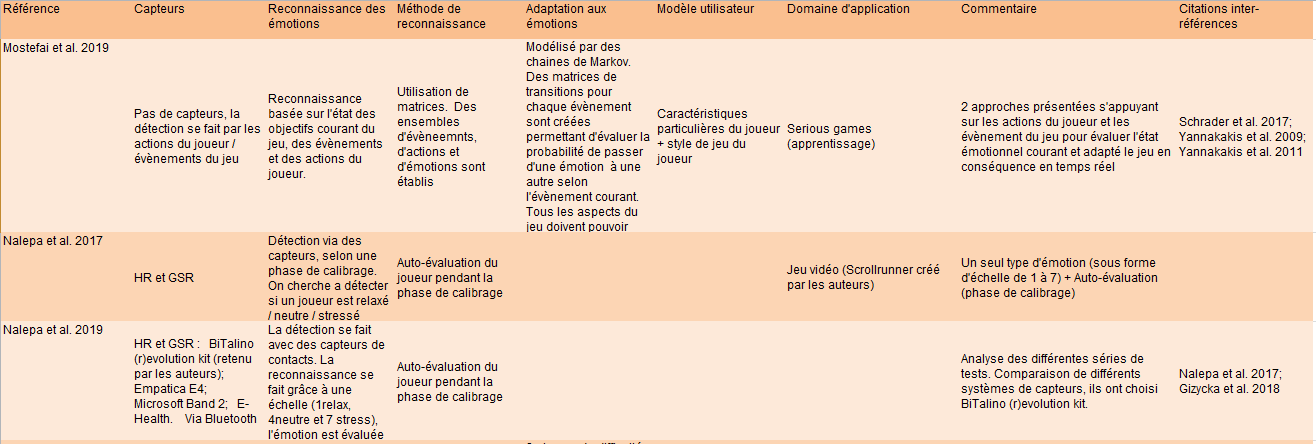
\includegraphics[scale=0.47]{include/tri1.PNG}
			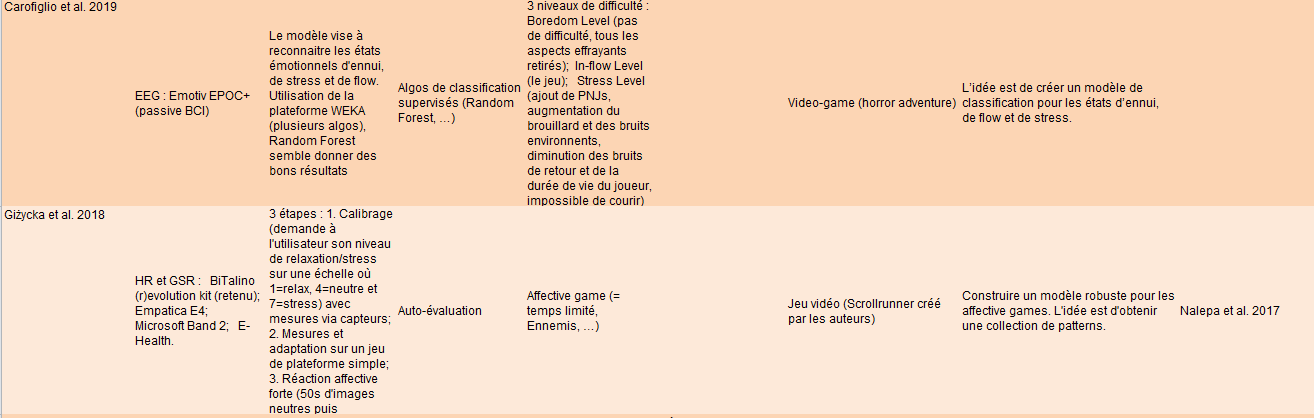
\includegraphics[scale=0.47]{include/tri2.PNG}
			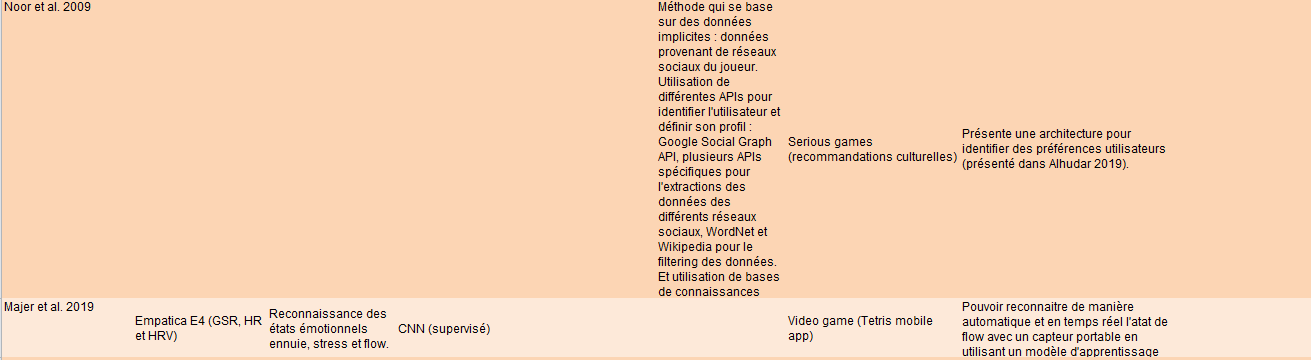
\includegraphics[scale=0.47]{include/tri3.PNG}
			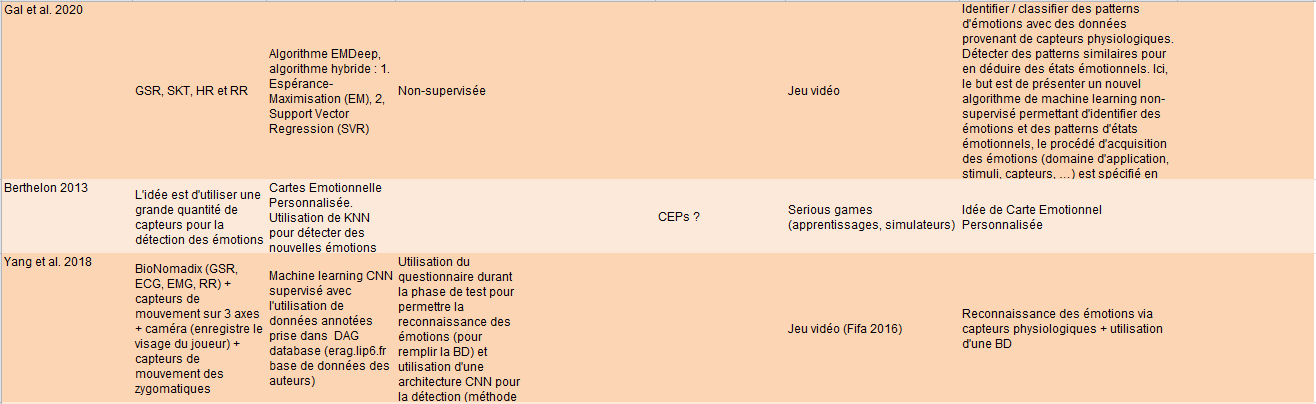
\includegraphics[scale=0.47]{include/tri4.PNG}
			\caption{Tableau synthétique des références (première partie)}
			\label{fig:tabsynt1}
		\end{figure}
		\begin{figure}
			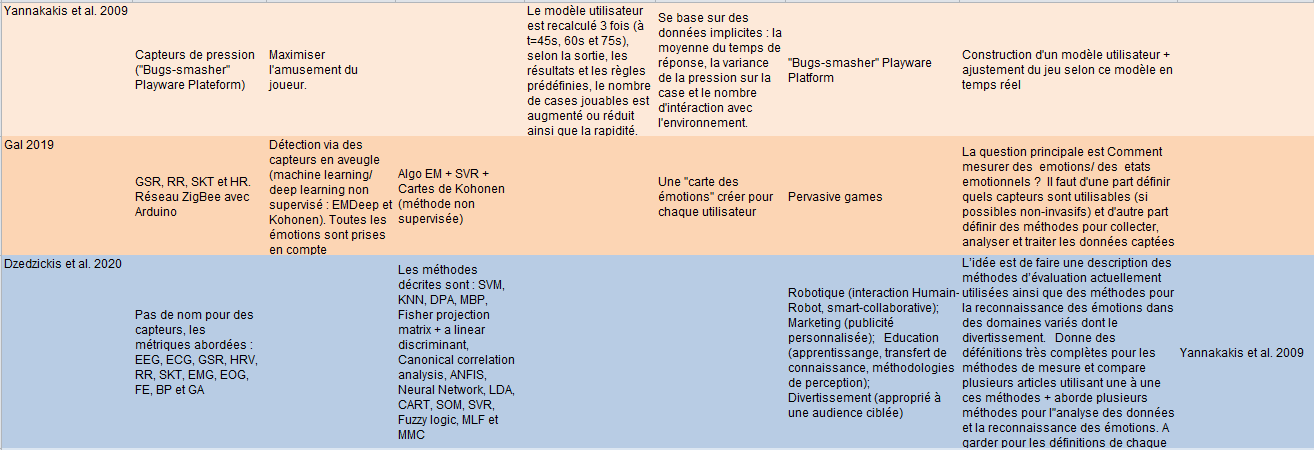
\includegraphics[scale=0.47]{include/tri5.PNG}
			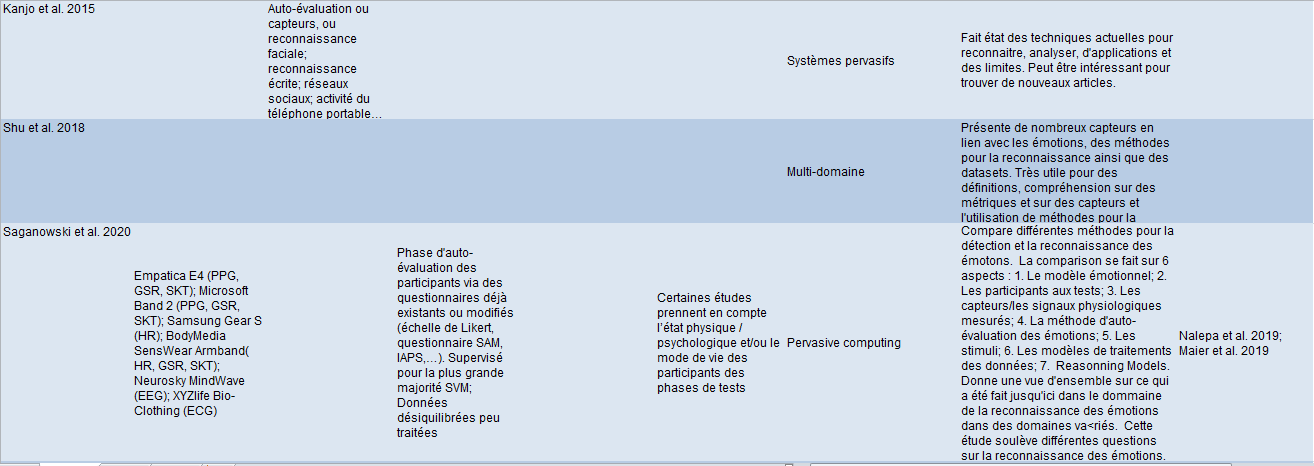
\includegraphics[scale=0.47]{include/tri6.PNG}
			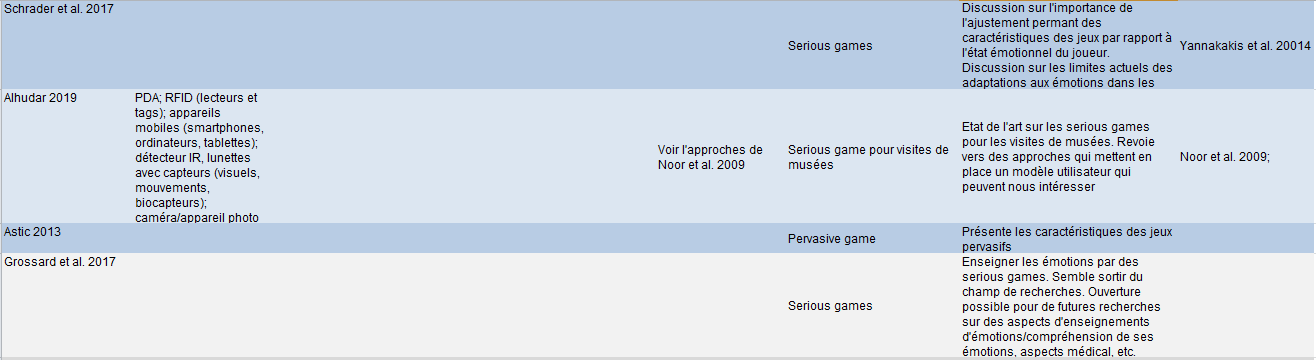
\includegraphics[scale=0.47]{include/tri7.PNG}
			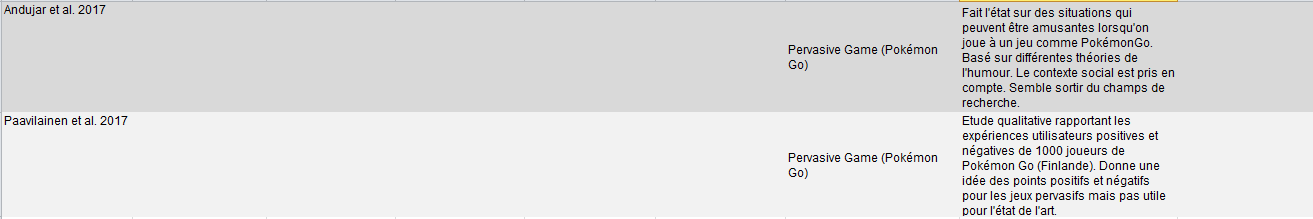
\includegraphics[scale=0.47]{include/tri8.PNG}
			\caption{Tableau synthétique des références (seconde partie)}
			\label{fig:tabsynt2}
		\end{figure}
		Ce tableau, que j'ai rempli et étoffé pendant mes recherches bibliographiques, mas aussi par la suite, m'a aidé à mieux comprendre les approches en catégorisant les méthodes et les expérimentations qui étaient décritent dans les références. 
		Ce tableau m'a également beaucoup aidé à transmettre les idées globales lors des réunions.\par
		A partir de fin avril, mes tuteur m'ont chargé de nouvelles missions. J'ai travaillé sur la rédaction d'un état de l'art et sur l'élaboration d'un modèle sous forme de diagramme de classe en parallèle.
	\subsection{Rédaction d'un état de l'art}
		J'ai dans un premier temps réfléchi à la problématique et à l'objectif que je voulais pour cet état de l'art. Mes tuteurs m'ont suggérés d'écrire une première introduction pour m'aider. Ce que j'ai fait.
		Ecrire cette introduction m'a permis de voir la direction que je souhaitais prendre.
		Après quelques correction de leur part, j'ai pu recentrer mes propos et mieux définir les idées que je voulais ransmettre.\par
		J'ai ensuite défini un plan que j'ai détaillé avec les points qui me semblait important à développer dans chaque partie. Je suis revenue plusieurs fois sur ce plan avec les correction et indications de mes tuteurs.\par
		Une fois que le plan m'a semblé pertinent, j'ai développé les parties.
	\subsection{Modélisation d'une ontologie}
	\subsection{Prototype avec l'environnement Kafka}

\section{Validation}

\section{Conclusion}


\newpage
\appendix
\section{Annexe 1 : Offre de stage}\label{app:annexe1}
	\textbf{Elaboration du modèle conceptuel des jeux pervasifs adaptables avec la prise en compte des états émotionnels des joueurs}\par
	\medskip
	\textbf{Contexte :}\newline
	Le champ des jeux affectifs est nouveau. Il s’appuie sur l’intégration de nouveaux moyens à développer dans les jeux afin d’adaptabilité. [1] et [2] présentent une méthodologie unifiée pour la conception des jeux affectifs utilisant le plus tôt possible le mécanisme de boucle émotionnelle. Ils repèrent des variations à l’aide de mesures physiologiques et appliquent un modèle issu d’un ensemble construit considéré comme en relation avec les émotions. Leur étude montre combien la dimension émotionnelle de l’utilisateur est importante mais difficile à gérer.\newline
	Le profil du joueur, y compris ses émotions, impacte la conception des jeux. Afin de proposer une meilleure expérience aux joueurs et de proposer un jeu particularisé, le jeu doit être adaptable en fonction du contexte global du joueur. Nous sommes dans une approche holistique qui combine à la fois l’individu et ses émotions, et, les influences de l’entourage qui va du bâtiment lui-même à l’atmosphère que dégage le lieu. Très peu de travaux ont été faits pour la conception et le développement des jeux adaptables dynamiquement. [3] formalise le concept des jeux appliqués aux visites de musées. Ce travail modélise le jeu de visite et propose un processus d’équilibrage entre la dimension ludique et la dimension non ludique (la visite) de ce type de jeux. [3] propose des patrons de mission qui servent d’éléments réutilisables lors de la conception des jeux, mais qui ne couvrent qu’une partie du processus de conception.\par
	\textbf{Sujet :}\newline
	Il s’agit dans ce stage d’élaborer un modèle conceptuel du jeu pervasif adaptable basé sur les émotions. Ce modèle, éventuellement réalisé sous forme d’une ontologie, doit couvrir toute la variété des facteurs qui impactent le jeu tels que le profil de l’utilisateur et ses données physiologiques exprimant son état émotionnel. Cette ontologie doit être construite de façon à ce qu’elle soit adaptée à la démarche situationnelle nécessaire pour la composition dynamique du jeu.



\bibliographystyle{abbrv}
\bibliography{include/biblio}
\end{document}